\documentclass[12pt]{report}
\usepackage{titlesec}
\usepackage{geometry} % Add the geometry package
\usepackage{graphicx}
\usepackage{titletoc}
\usepackage{blindtext}
\usepackage{longtable}
\usepackage{enumitem}
\usepackage{tabularx}
\usepackage{float}
\usepackage{xcolor}
\usepackage[document]{ragged2e}
\usepackage{etoolbox}
\usepackage{tikz} % Include the tikz package for drawing

\usepackage{todonotes}                          %ENTFERNEN, WENN DOKUMENT FERTIG UM ALLE TO-DOs ZU ÜBERPRÜFEN
\usepackage{blindtext}                          %Lorem ipsum... ENTFERNEN, WENN DOKUMENT FERTIG UM ALLE BLINDTEXTE ZU ÜBERPRÜFEN


\makeatletter
\patchcmd{\chapter}{\if@openright\cleardoublepage\else\clearpage\fi}{}{}{}
\makeatother

 %Redefine the \chapter command to include custom chapter names with numbers
\makeatletter
\newcommand{\customchapter}[1]{%
 \refstepcounter{chapter}%
\chapter*{\thechapter. #1}%
  \addcontentsline{toc}{chapter}{\thechapter. #1}%
  
}
\makeatother

 %Customize the chapter heading format
%\titleformat{\chapter}[display]
 % {\normalfont\huge\bfseries}
  %{0pt}
  %{0pt}
  %{\LARGE}

% Configure page layout with the geometry package
\geometry{
  left=.75in,  % Adjust the left margin
  right=.75in, % Adjust the right margin
  top=.75in,   % Adjust the top margin
  bottom=.75in % Adjust the bottom margin
}

% Customize the spacing above and below chapter titles
\titlespacing*{\chapter}{0pt}{0pt}{10pt} % Adjust the last value (10pt) to control the space

\begin{document}

\begin{titlepage}
\begin{center}
    \hspace{5mm}\textbf{\LARGE Lab Oriented Project Report }
    \begin{center}
    \vspace{0.5mm}
    \Large On
    \end{center}
    \vspace{0.5mm}
    \center{\textbf{\LARGE Final Specification}}
\end{center}

\vspace{5mm}
\begin{center}
\textcolor{darkgray}{\LARGE Submitted in partial fulfilment }
\end{center}
\begin{center}
\vspace{0.5mm}
\Large of
\vspace{0.5mm}
\end{center}
\begin{center}
\textbf{\LARGE Computer Architecture}
\end{center}

\vspace{5mm}

\begin{figure}[h!]
    \begin{center}
    
\includegraphics[width=10cm, height=3cm]{Image/logoR.png}
    \end{center}
    \end{figure}
    
\vspace{2mm} 
\begin{center}
\textbf{\Large Under the Guidance of :}
\newline
\Large Prof. Dr. A. Siggelkow 
\end{center}

\vspace{5mm}

\textbf{\hspace{70mm} \Large Submitted By :}

\hspace{63mm} \Large Jayant Patil (18041745)
\par
\hspace{60mm} \Large Aditya Grewal (29541041)
\par
\hspace{57mm} \Large Avanindra Kumar Mishra (20241804) 
\par 
\hspace{47mm} \Large Sagar Shreeshailappa Hosmani (27741741)

\hspace{47mm} \Large Omkarnimith Muthabyraiah(16841822)
\par
\hspace{65mm} \Large Jash Shah (23741845)
% Author
%{ \large
 % {\textit{\textbf{Guided by}}}, \\[0.1cm]
  %}
  % \Large
  %\textbf{Prof. Dr.-Ing. A. Siggelkow }\\[0.1cm]
%}

\vspace{5mm}
\begin{center}

\textbf{\Large MASTER OF ELECTRICAL ENGINEERING AND EMEBDDED SYSTEMS}\\[0.4cm]
\vspace{5mm}
\textbf{\Large HOCHSCHULE RAVENSBURG-WEINGARTEN}\\[0.4cm]
% Bottom
\vspace{5mm}
\textbf{\Large \today}
\end{center}
 \end{titlepage}


	
	
	\tableofcontents 
 \newpage
	\listoffigures
	\listoftables
	%\section*{Glossary}
	%\section*{Naming Conventions}
	%\section*{Document List}

\newpage
\customchapter{Functional Requirements}
\begin{longtable}{|p{3.5cm}|p{1cm}|p{2.5cm}|p{2cm}|p{6.5cm}|}
 \hline
 \textbf{Requirement} & \textbf{ID} & \textbf{Importance} & \textbf{Verifiable} & \textbf{Description} \\
 \hline
 \hline
Program Counter (PC) & G01 & High & System Verilog-TB &The PC holds the address of the next instruction to be executed. It increments by 4 bytes each clock cycle, corresponding to the size of each instruction.
\\
 \hline
  Instruction Memory & G02 & High & System Verilog-TB & Stores the program's instructions and supplies them to the processor. It retrieves instructions based on the address provided by the PC.
\\
\hline
Instruction Decoder & G03 & High & System Verilog-TB & Interprets the binary instruction fetched from the instruction memory. It generates control signals to guide the processor components.
\\
    
 \hline
 Register File & G05 & High & System Verilog-TB & Consists of 32 general-purpose registers for storing intermediate data and results. It supports two read ports and one write port.
\\
\hline
 Arithmetic Logic Unit (ALU) & G06 & High & System Verilog-TB & Performs arithmetic and logical operations. Receives operands from the register file or immediate values and executes operations specified by control signals.
\\
\hline
 Data Memory & G07 & High & System Verilog-TB & Used for reading from and writing to memory locations during load and store instructions. It interacts with memory beyond the register file. 
  \\
 \hline
 Control Unit & G08 & High & System Verilog-TB & Generates control signals based on the decoded instruction. Directs operations of the ALU, data memory, and register file.\\
 \hline
  Instruction Execution Flow & G08 & High & System Verilog-TB & Each instruction starts by using the PC to fetch the instruction. Operands are read from the registers. The ALU is used for address calculation, operation execution, or equality check. Results are written back to the register file or used for further processing.\\
 \hline
  Memory-Reference Instructions & G08 & High & System Verilog-TB & Includes load doubleword (ld) and store doubleword (sd). Uses the ALU for address calculation and accesses memory for data operations.\\
 \hline
  Arithmetic-Logical Instructions & G08 & High & System Verilog-TB & Includes add, sub, and, and or. Uses the ALU for executing operations and writes results back to registers.\\
 \hline
  Conditional Branch Instructions & G08 & High & System Verilog-TB & Includes branch if equal (beq). Uses the ALU for equality tests and may alter the next instruction address based on the comparison.\\
 \hline
  Multiplexors & G08 & High & System Verilog-TB & Regulate the flow of data to various components based on the instruction class. Controlled by control signals decoded from the instruction.\\
 \hline

 RISC-V RV64I Compliance & G08 & High & Application Program & The processor must support all RV64I instructions (e.g., ADD, LOAD, STORE, BEQ) and execute them correctly as per the RISC-V specifications.\\
 \hline
\end{longtable}

 \newpage
\customchapter{History}

\begin{table}[H]
	\centering
	\begin{tabular}{|p{2cm}|p{2.3cm}|p{5.5cm}|p{6cm}|}
		\hline
		\textbf{Rev. No.} & \textbf{Rev. Date} & \textbf{Description of change in Current Version} & \textbf{Author}\\
		\hline
		\hline
		V 1.0 & 15.04.2024 & Functional Requirements & Jayant Patil \newline Aditya Grewal \newline Avanindra Kumar Mishra \newline Omkarnimith Muthabyraiah \newline Jash Shah \newline Sagar Shreeshailappa Hosmani\\
		\hline
		V 2.0 & 05.06.2024 & Specifications & Jayant Patil \newline Aditya Grewal \newline Avanindra Kumar Mishra \newline Omkarnimith Muthabyraiah \newline Jash Shah \newline Sagar Shreeshailappa Hosmani\\
		\hline
		V 3.0 & 15.06.2024 & Final Specifications, Design Descriptions and Simulation & Jayant Patil \newline Aditya Grewal \newline Avanindra Kumar Mishra \newline Omkarnimith Muthabyraiah \newline Jash Shah \newline Sagar Shreeshailappa Hosmani\\
		\hline
	\end{tabular}
\end{table}

\newpage
\customchapter{Document Overview}
\section{Glossary}
\begin{table}[H]
    \centering
    \begin{tabularx}{\textwidth}{|p{3cm}|X|}
        \hline
        \textbf{Term} & \textbf{Description} \\
        \hline\hline
        ALU (Arithmetic Logic Unit) & A digital circuit used to perform arithmetic and logical operations. In the RISC-V implementation, the ALU performs operations such as addition, subtraction, AND, and OR based on the control signals provided. \\
        \hline
        ALU Control & The unit that generates the control signals for the ALU based on the ALUOp field and the function codes (funct7 and funct3) of the instruction. It determines which operation the ALU will perform. \\
        \hline
        ALUOp & A 2-bit control signal that indicates the type of operation to be performed by the ALU. The values of ALUOp determine whether the operation is an addition, subtraction, or a function determined by the funct7 and funct3 fields for R-type instructions. \\
        \hline
        Branch & A control signal indicating whether the current instruction is a branch instruction. If the condition for the branch is met, the program counter (PC) is updated to the target address. \\
        \hline
        Control Unit & The component that generates control signals based on the opcode of the instruction. It orchestrates the flow of data within the CPU, enabling the execution of instructions by controlling the operation of other components such as the ALU, registers, and memory. \\
        \hline
        Data Memory & A memory unit used to store data during program execution. The data memory is accessed using addresses computed by the ALU, and it supports read and write operations. \\
        \hline
        Immediate Generator (ImmGen) & A unit that generates immediate values from the instruction fields. Immediate values are often used for arithmetic operations or as addresses for load and store instructions. \\
        \hline
        Instruction Memory & A memory unit that stores the program instructions. The instruction memory is accessed sequentially using the program counter (PC), which holds the address of the current instruction. \\
        \hline
        MUX (Multiplexer) & A digital switch that selects one of several input signals and forwards the selected input to the output. In the RISC-V implementation, MUXes are used to select between different data sources based on control signals. \\
        \hline
        Program Counter (PC) & A register that holds the address of the next instruction to be executed. The PC is updated after each instruction fetch to point to the next instruction in memory. \\
      
        \hline
    \end{tabularx}
\end{table}

\newpage

\begin{table}[H]
    \centering
    \begin{tabularx}{\textwidth}{|p{3cm}|X|}
        \hline
        \textbf{Term} & \textbf{Description} \\
        \hline\hline
        Register File & A set of registers used to store operands and intermediate results. The register file has read and write ports to access and update the registers during instruction execution. \\
        \hline
        Zero Flag & A flag set by the ALU to indicate whether the result of an operation is zero. This flag is often used for branch instructions to determine if a condition is met (e.g., branch if equal). \\
        \hline
        Funct3 and Funct7 & Fields within the R-type instruction format that specify the specific operation to be performed by the ALU. Funct3 is a 3-bit field, and funct7 is a 7-bit field. \\
        \hline
        MemRead & A control signal that enables reading data from memory. \\
        \hline
        MemWrite & A control signal that enables writing data to memory. \\
        \hline
        MemtoReg & A control signal that determines whether the data to be written to a register comes from memory or the ALU result. \\
        \hline
        RegWrite & A control signal that enables writing data to a register in the register file. \\
        \hline
        ALUSrc & A control signal that determines whether the second operand for the ALU comes from a register or an immediate value. \\
        \hline
        Add & An arithmetic operation where two values are summed. In the context of the PC, adding 4 to the current PC value points to the next instruction. \\
        \hline
        Shift Left 1 & An operation that shifts a binary value left by one position, effectively multiplying it by 2. This operation is often used in calculating branch target addresses. \\
        \hline
    \end{tabularx}
    \caption{Glossary of Terms for RISC-V Implementation}
    \label{tab:glossary}
\end{table}



\newpage
\customchapter{Product Overview}
The RV64I single-cycle RISC-V processor is a fundamental design that exemplifies simplicity and efficiency in modern computer architecture. This processor, which adheres to the RISC-V instruction set architecture (ISA), is characterized by its 64-bit width and single-cycle execution, where each instruction is completed in one clock cycle.\\
\vspace{\baselineskip}
\textbf{Fundamental design elements in RV64I are:}
\begin{itemize}
\item \textbf{The Program Counter (PC)} is a crucial component that holds the address of the next instruction to be executed in the sequence. On each clock cycle, the PC increments by 4 bytes, corresponding to the size of each instruction in the RISC-V architecture.
\item \textbf{Instruction Memory} is responsible for storing the program's instructions and supplying them to the processor. When the PC provides an address, the instruction memory retrieves the corresponding instruction and forwards it to the instruction decoder. This read-only memory is typically implemented as a ROM or a similar non-volatile storage, ensuring the integrity and availability of the program instructions throughout the execution cycle.
\item \textbf{The Instruction Decoder} plays a pivotal role in interpreting the binary instruction fetched from the instruction memory. It breaks down the instruction into its constituent parts, such as opcode, source registers, destination register, and immediate values. The decoder then generates the necessary control signals that guide the other components of the processor to perform the specified operation, whether it be an arithmetic calculation, memory access, or control flow alteration.
\item \textbf{The Register File} consists of a set of 32 general-purpose registers that store intermediate data and results during instruction execution. It includes two read ports and one write port, allowing two source operands to be read simultaneously and one result to be written back each cycle.
\item \textbf{The Arithmetic Logic Unit (ALU)} is the computational heart of the processor, responsible for performing arithmetic operations (such as addition, subtraction) and logical operations (such as AND, OR, XOR). The ALU receives its operands from the register file or immediate values decoded from the instruction and executes the operation specified by the control signals from the instruction decoder. The result is then either written back to a register or used for further processing.
\item \textbf{Data Memory} is used for reading from and writing to memory locations during load and store instructions. The memory address is calculated by the ALU and sent to the data memory along with the data to be stored (for store operations) or a request to retrieve data (for load operations). This allows the processor to interact with memory to access data beyond the limited capacity of the register file, enabling larger and more complex computations.
\item \textbf{The Control Unit} generates the necessary control signals based on the decoded instruction. These signals direct the operation of other components like the ALU, data memory, and register file. It determines the type of operation (arithmetic, logical, load, store, branch) and configures the processor’s pathways accordingly.
\end{itemize}
Our design is capable of executing memory-reference instructions load doubleword (ld) and store doubleword (sd), the arithmetic-logical instructions add, sub, and, and or, and the conditional branch instruction branch if equal (beq).\\
\vspace{\baselineskip}
\textbf{For every instruction, the first two steps are identical:}
\begin{itemize}
\item Send the program counter (PC) to the memory that contains the code and fetch the instruction from that memory.
\item Read one or two registers, using fields of the instruction to select the registers to read. For the ld instruction, we need to read only one register, but most other instructions require reading two registers.
\end{itemize}
After these two steps, the actions required to complete the instruction depend on the instruction class. The three instruction classes involved in this design are memory-reference, arithmetic-logical, and branches. All instruction classes use the arithmetic-logical unit (ALU) after reading the registers. The memory-reference instructions use the ALU for an address calculation, the arithmetic logical instructions for the operation execution, and conditional branches for the equality test. After using the ALU, the actions required to complete various instruction classes differ. A memory reference instruction will need to access the memory either to read data for a load or write data for a store. An arithmetic-logical or load instruction must write the data from the ALU or memory back into a register. Lastly, for a conditional branch instruction, we may need to change the next instruction address based on the comparison; otherwise, the PC should be incremented by four to get the address of the subsequent instruction.\\
\vspace{\baselineskip}
Below figure shows the high-level view of a RISC-V implementation, focusing on the various functional units and their interconnection along with the required multiplexors as well as control lines for the major functional units.
 \begin{figure}[H]
    \centering
    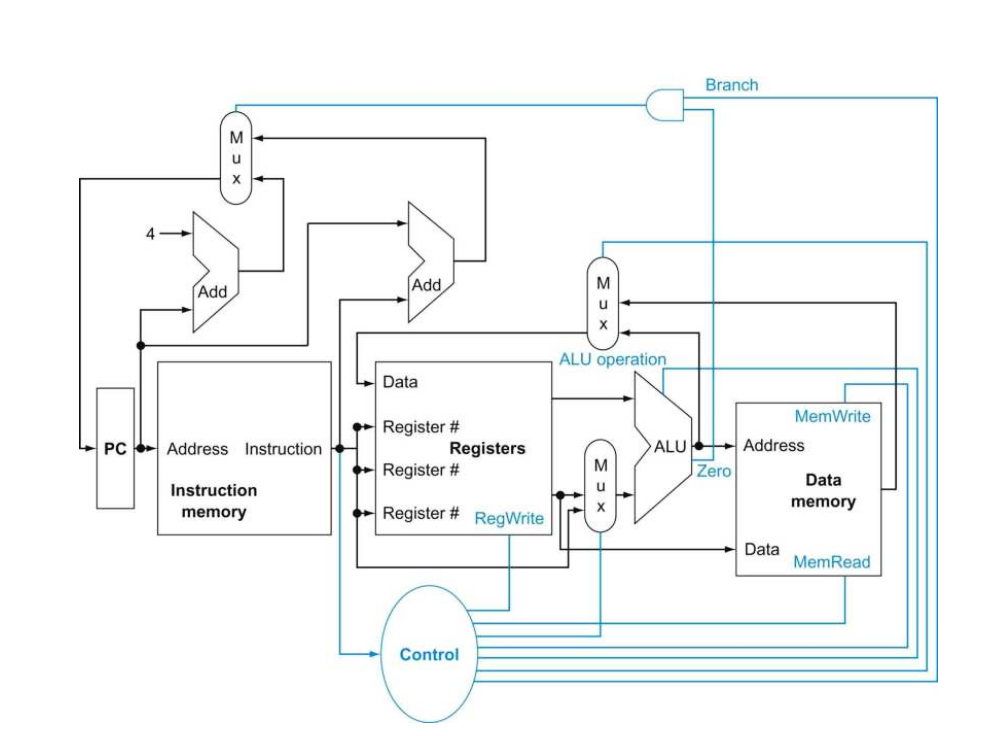
\includegraphics[width=0.8\linewidth]{Image/Abstract.png}
    \caption{Abstract view of RV64I}
    \label{fig:enter-label}
\end{figure}
All instructions start by using the program counter to supply the instruction address to the instruction memory. After the instruction is fetched, the register operands used by an instruction are specified by fields of that instruction. Once the register operands have been fetched, they can be operated on to compute a memory address (for a load or store), to compute an arithmetic result (for an integer arithmetic-logical instruction), or an equality check (for a branch). If the instruction is an arithmetic-logical instruction, the result from the ALU must be written to a register. If the operation is a load or store, the ALU result is used as an address to either store a value from the registers or load a value from memory into the registers. The result from the ALU or memory is written back into the register file. Branches require the use of the ALU output to determine the next instruction address, which comes either from the adder (where the PC and branch offset are summed) or from an adder that increments the current PC by four. The thick lines interconnecting the functional units represent buses, which consist of multiple signals. The arrows are used to guide the reader in knowing how information flows. Since signal lines may cross, we explicitly show when crossing lines are connected by the presence of a dot where the lines cross.\\
\vspace{\baselineskip}
The multiplexors are used to regulate the flow of the data to various design elements depending on the class of the instruction that is being executed. These multiplexors are controlled by various control signals decoded from the instruction itself. A detailed description of the instruction decoding, control signals, datapath and other necessary design elements will be given in detail in Chapter 6.
\newpage
\vspace*{-2cm} % Adjust the value as needed
\customchapter{Architecture Concepts}

\section{RISC-V ISA}
The RISC-V ISA (Instruction Set Architecture) is a modern, open standard developed to support a wide range of computing devices. The RV64I is a specific implementation of the RISC-V ISA, focusing on a 64-bit integer base instruction set. The RV64I ISA is a simple yet powerful 64-bit instruction set designed with a reduced instruction set computing (RISC) philosophy. It includes a basic set of instructions for integer computation, memory operations, and control flow, which form the foundation for more complex instructions and extensions.\\
\vspace{\baselineskip}
RV64I defines 32 general-purpose registers (x0 to x31), each 64 bits wide. Register x0 is hardwired to zero, providing a convenient way to zero out registers or perform no-ops in certain instructions. The other registers (x1 to x31) are used for standard data manipulation and addressing.

\subsection{Instruction Formats}
RV64I uses a fixed 32-bit instruction format with several encoding types to support various instruction needs:
\begin{table}[h]
\centering
\begin{tabular}{|>{\centering\arraybackslash}m{2cm}|>{\centering\arraybackslash}m{3cm}|>{\centering\arraybackslash}m{1cm}|>{\centering\arraybackslash}m{1cm}|>{\centering\arraybackslash}m{1.3cm}|>{\centering\arraybackslash}m{3cm}|>{\centering\arraybackslash}m{1.5cm}|>{\centering\arraybackslash}m{3cm}|}
\hline
\textbf{Name} \newline \textbf{(Field size)} & \textbf{7 bits} & \textbf{5 bits} & \textbf{5 bits} & \textbf{3 bits} & \textbf{5 bits} & \textbf{7 bits} & \textbf{Comments} \\
\hline
R-type & funct7 & rs2 & rs1 & funct3 & rd & opcode & Arithmetic instruction format \\
\hline
I-type & \multicolumn{2}{c|}{immediate[11:0]} & rs1 & funct3 & rd & opcode & Loads \& immediate arithmetic \\
\hline
S-type & immed[11:5] & rs2 & rs1 & funct3 & immed[4:0] & opcode & Stores \\
\hline
SB-type & immed[12,10:5] & rs2 & rs1 & funct3 & immed[4:1,11] & opcode & Conditional branch format \\
\hline
U-type & \multicolumn{4}{c|}{immediate[20,10:1,11,19:12]} & rd & opcode & Unconditional jump format \\
\hline
UJ-type & \multicolumn{4}{c|}{immediate[31:12]} & rd & opcode & Upper immediate format \\
\hline
\end{tabular}
\caption{RISC-V Instruction Formats}
\end{table}
\begin{itemize}
\item \textbf{R-Type (Register-Register):} Used for arithmetic and logical operations between registers.
\item \textbf{I-Type (Immediate):} Used for arithmetic operations with an immediate value, loads, and certain control instructions.
\item \textbf{S-Type (Store):} Used for storing data from a register to memory.
\item \textbf{SB-Type (Branch):} Used for conditional branching based on comparisons between register values.
\item \textbf{U-Type (Upper Immediate):} Used for instructions that operate with a 20-bit upper immediate.
\end{itemize}
In our design, we will only be implementing datapaths and logic elements for R-Type, I-Type, S-Type and SB-Type instruction classes.
 
\newpage
\customchapter{Description of the Design Elements}

\section{Register File}

\subsection{Overview}
The register file is a fundamental component in the RISC-V processor architecture, responsible for providing fast storage and access to the CPU's general-purpose registers. This module is integral to the CPU's operation, enabling efficient data handling and manipulation during instruction execution.

\subsection{Architectural Design}
A register file consists of a set of registers that can be read and written by specifying the register number. The RISC-V architecture typically uses a register file with 32 registers, each 64 bits wide in the RV64I subset. This allows for rapid data access and storage, crucial for maintaining high performance in processing tasks.

The register file is designed to support multiple read and write operations. Specifically, it includes:
\begin{itemize}
    \item Two read ports, allowing simultaneous reading from two registers.
    \item One write port, enabling the writing of data to a single register per clock cycle.
\end{itemize}

\begin{figure}[h]
\centering
\hspace*{2cm} % Indentation
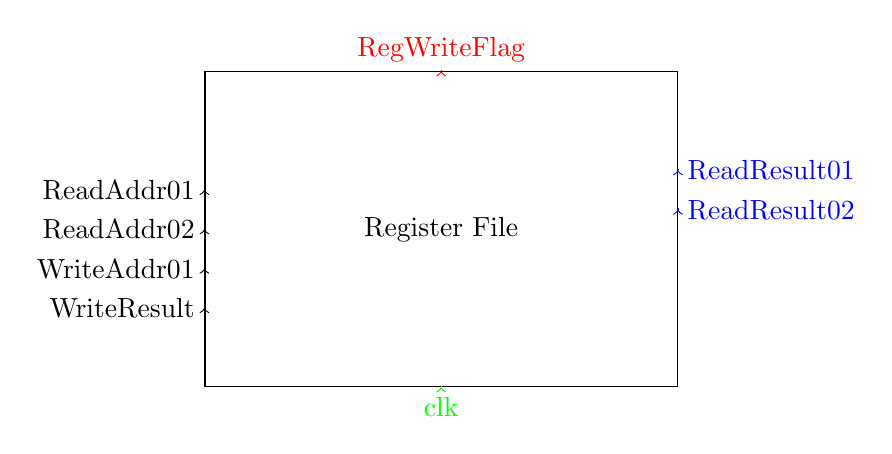
\begin{tikzpicture}
    % Register File Block
    \node[draw, rectangle, minimum width=6cm, minimum height=4cm] (regfile) {Register File};

    % Inputs
    \node[anchor=south, text=red] (regwrite) at (regfile.north) {RegWriteFlag};
    \node[anchor=east] (readaddr1) at (regfile.west |- 1, 0.5) {ReadAddr01};
    \node[anchor=east] (readaddr2) at (regfile.west |- 2, 0) {ReadAddr02};
    \node[anchor=east] (writeaddr) at (regfile.west |- 3, -0.5) {WriteAddr01};
    \node[anchor=east] (writeresult) at (regfile.west |- 4, -1) {WriteResult};
    \node[anchor=north, text=green] (clk) at (regfile.south) {clk};

    % Outputs
    \node[anchor=west, text=blue] (readresult1) at (regfile.east |- 1, 0.75) {ReadResult01};
    \node[anchor=west, text=blue] (readresult2) at (regfile.east |- 2, 0.25) {ReadResult02};

    % Arrows
    \draw[->, red] (regwrite.south) -- (regfile.north);
    \draw[->] (readaddr1.east) -- (regfile.west |- 1, 0.5);
    \draw[->] (readaddr2.east) -- (regfile.west |- 2, 0);
    \draw[->] (writeaddr.east) -- (regfile.west |- 3, -0.5);
    \draw[->] (writeresult.east) -- (regfile.west |- 4, -1);
    \draw[->, green] (clk.north) -- (regfile.south);
    \draw[->, blue] (regfile.east |- 1, 0.75) -- (readresult1.west);
    \draw[->, blue] (regfile.east |- 2, 0.25) -- (readresult2.west);
\end{tikzpicture}
\caption{Register File Block Diagram}
\end{figure}

\subsection{Functional Operation}
In the context of the RISC-V CPU, the register file interacts closely with other components such as the ALU (Arithmetic Logic Unit) and instruction decoder. During the execution of R-format instructions, for example, the register file provides the operands for the ALU and stores the result of the computation.

The typical operations involving the register file include:
\begin{enumerate}
    \item \textbf{Read Operations}: Two source registers are read, and their values are provided to the ALU or other computational units.
    \item \textbf{Write Operations}: The result of an ALU operation or a value loaded from memory is written back to a destination register.
\end{enumerate}

The design ensures that reads are combinational operations, meaning the data is immediately available based on the provided register addresses. Writes, however, are sequential operations controlled by a clock signal to ensure data integrity and proper synchronization.

\subsection{Integration with CPU Architecture}
The register file is crucial for the overall performance of the CPU as it stores the operands and results of arithmetic and logic operations. It interfaces directly with the instruction memory, instruction decoder, and the ALU:
\begin{itemize}
    \item \textbf{Instruction Memory}: The instruction memory fetches instructions that specify which registers to read from and write to.
    \item \textbf{Instruction Decoder}: The decoder interprets the instructions and generates control signals required to access the register file.
    \item \textbf{ALU}: The ALU performs computations using the data read from the register file and stores the results back into the register file.
\end{itemize}

\begin{figure}[h]
\centering
\hspace*{2cm} % Indentation
\begin{tikzpicture}
    % Blocks
    \node[draw, rectangle, minimum width=3cm, minimum height=1.5cm] (instmem) {Instruction Memory};
    \node[draw, rectangle, minimum width=3cm, minimum height=1.5cm, below=1cm of instmem] (instdec) {Instruction Decoder};
    \node[draw, rectangle, minimum width=3cm, minimum height=1.5cm, below=1cm of instdec] (regfile) {Register File};
    \node[draw, rectangle, minimum width=3cm, minimum height=1.5cm, below=1cm of regfile] (alu) {ALU};
    \node[draw, rectangle, minimum width=3cm, minimum height=1.5cm, right=4cm of regfile] (datamem) {Data Memory};

    % Arrows
    \draw[->] (instmem.south) -- (instdec.north);
    \draw[->] (instdec.south) -- (regfile.north);
    \draw[->] (regfile.south) -- (alu.north);
    \draw[<->] (alu.east) -- (datamem.west);
    \draw[->] (alu.west) -- ++(-1,0) node[midway, above] {Result} -- ++(0,2.5) -- (regfile.west);

\end{tikzpicture}
\caption{Integration of Register File within the CPU}
\end{figure}

\subsection{Initialization and Read/Write Synchronization}
In practical implementations, some registers in the register file may be initialized to specific values for various purposes, such as testing or specific algorithmic requirements. This initialization can be crucial for certain applications or during the boot process of the CPU.

The read operations are usually instantaneous, providing the required data to the ALU or other processing units without delay. Write operations are synchronized with the clock to ensure data integrity and prevent race conditions.

\subsection{Signal Descriptions}
The key signals associated with the register file include:
\begin{itemize}
    \item \textbf{clk}: The clock signal that synchronizes the write operations.
    \item \textbf{regWriteFlag}: A control signal indicating whether a write operation should be performed.
    \item \textbf{readAddr01, readAddr02}: Addresses of the registers to be read.
    \item \textbf{writeAddr01}: Address of the register to be written.
    \item \textbf{writeResult}: Data to be written to the specified register.
    \item \textbf{readResult01, readResult02}: Data read from the specified registers.
\end{itemize}

\subsection{Conclusion}
The register file is a crucial part of the RISC-V processor, enabling efficient and fast access to frequently used data. Its design supports simultaneous reads and controlled writes, ensuring high performance and reliability. Understanding the operation and integration of the register file within the processor architecture is essential for implementing and optimizing RISC-V systems.


\newpage
\section{ALU}

This module is a behavioral model of an Arithmetic Logic Unit (ALU) for a RISC-V  processor implemented in SystemVerilog. This ALU performs various arithmetic and logic operations based on the provided control signals. The module takes two 64-bit input operands and produces a 64-bit result. It also generates a zero flag to indicate whether the result is zero.

\subsection{Ports}

\begin{itemize}
    \item data01 (input, 64 bits): The first operand for the ALU operation.
    \item data02 (input, 64 bits): The second operand for the ALU operation.
    \item aluCtl (input, 4 bits): The control signal to specify the type of operation to be performed.
    \item aluOp (input, 2 bits): The high-level operation type signal, used for decoding the instruction class.
    \item zeroFlag (output, 1 bit): A flag that indicates whether the result is zero.
    \item result (output, 64 bits): The result of the ALU operation.
\end{itemize}



\begin{figure}[H]
    \centering
    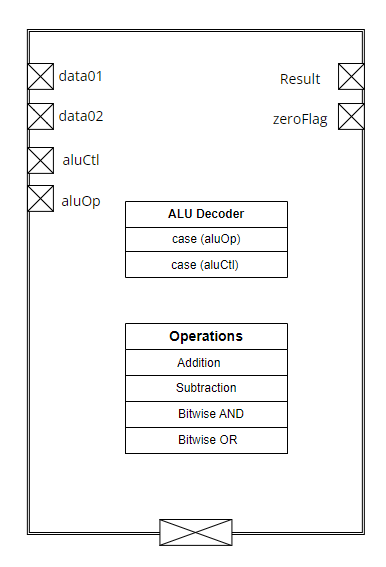
\includegraphics[width=0.4\linewidth]{Image/Block Diagram.png}
    \caption{ALU block diagram}
    \label{fig:ALU block diagram}
\end{figure}

\subsection{Parameters}
\begin{itemize}
    \item \textbf{loadOrStoreOp (2 bits):} Specifies load or store operation (2'b00).
    \item \textbf{branchOp (2 bits):} Specifies branch operation (2'bx1).
    \item \textbf{rTypeOp (2 bits)}: Specifies R-type operation (2'b1x).
    \item \textbf{store (4 bits): }Specifies store operation (4'b0010).
    \item \textbf{load (4 bits):} Specifies load operation (4'b0010).
    \item \textbf{branchIfEqual (4 bits):} Specifies branch if equal operation (4'b0110).
    \item \textbf{ariAdd (4 bits):} Specifies addition operation (4'b0010).
    \item \textbf{ariSub (4 bits):} Specifies subtraction operation (4'b0110).
    \item \textbf{bitAnd (4 bits):} Specifies bitwise AND operation (4'b0000).
    \item \textbf{bitOr (4 bits):} Specifies bitwise OR operation (4'b0001).
\end{itemize}

\subsection{ ALU Operation}
The ALU operation is decoded based on the aluOp and aluCtl signals. The following table summarizes the operations.



\begin{figure}[H]
    \centering
    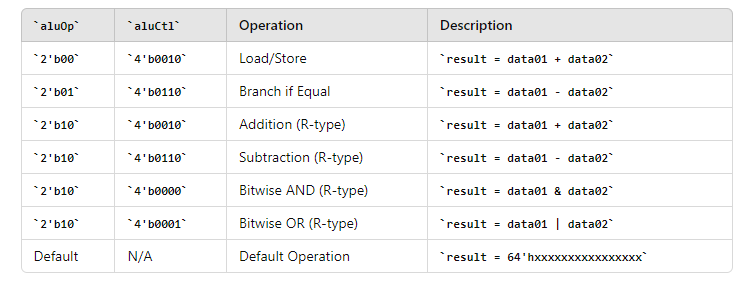
\includegraphics[width=0.5\linewidth]{Image/Alu truth table.png}
    \caption{ALU operation truth table}
    \label{fig:ALU operation truth table}
\end{figure}


\subsection{Detailed Functionality}
\begin{enumerate}
    \item Load/Store Operation (aluOp = 2'b00)
     \begin{itemize}
    \item Performs addition of data01 and data02.
     \item Sets zeroFlag if the result is zero.
     \end{itemize}
    
    \item Branch Operation (aluOp = 2'bx1)
    \begin{itemize}
     \item Performs subtraction of data01 and data02.
     \item Sets zeroFlag if the result is zero, indicating equality.
     \end{itemize}
     
    \item R-type Operation (aluOp = 2'b1x)
           \begin{itemize}
     \item Addition (aluCtl = 4'b0010): Adds data01 and data02.
    \item Subtraction (aluCtl = 4'b0110): Subtracts data02 from data01.
    \item Bitwise AND (aluCtl = 4'b0000): Performs bitwise AND between data01 and data02.
     \item Bitwise OR (aluCtl = 4'b0001): Performs bitwise OR between data01 and data02.
     \item Sets zeroFlag if the result of any operation is zero.
     \end{itemize}
    
    \item Default Operation
      \begin{itemize}
     \item Sets result to 64'hxxxxxxxxxxxxxxxx.
     \item Sets zeroFlag to 0.
     \end{itemize}
\end{enumerate}
\section{Instruction memory}
\subsubsection{Overview}
To execute any operation, the first step involves fetching the instruction from memory. To prepare for the next instruction, we increment the program counter so it points to the subsequent instruction's address, typically advancing by 4 bytes. This setup forms a datapath that handles instruction fetching and program counter incrementation for sequential instruction execution.

\subsubsection{Design Requirements}
\begin{itemize}
    \item \textbf{Memory Size:} 128 bytes (32 32-bit instructions). 
    \item \textbf{Data Bus Widths:}
    \begin{itemize}
    \item \textbf{Program Counter (PC):} 64 bits
    \item \textbf{Flash Instruction Input (flashInstruction):} 8 bits
    \item \textbf{Instruction Output: } 32 bits
    \item \textbf{Program Counter Bypass Output (pcBypass): } 64 bits 
    %\begin{tikzpicture}[baseline={([yshift=-.8ex]current bounding box.center)}]
   
    \end{itemize}
    \begin{figure}[H]
    \centering
    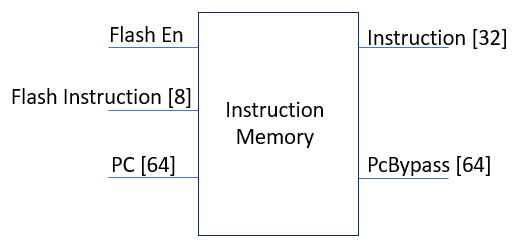
\includegraphics[width=0.5
    \linewidth]{Image/Instruction_Memory.png}
    \caption{Instruction Memory}
    \label{fig:enter-label}
\end{figure}
\end{itemize}
\subsubsection{Implementation Approach}
The implementation approach for the instructionMemory module involves the following key components and strategies:
\begin{itemize}
    \item \textbf{Memory Array:} A 128-byte internal memory array (instructionMem) is used to store the instructions. Each byte in this array represents a portion of the stored instructions.
    \item \textbf{Conditional Operation:} The module uses conditional logic to switch between flash programming mode and instruction fetch mode based on the state of the flashEn signal. This is achieved through a combination of always blocks and conditional assignments.
    \item \textbf{Byte Concatenation:} During instruction fetch mode, the module concatenates four consecutive bytes from the memory array to form a 32-bit instruction. This ensures that the CPU can retrieve complete instructions for execution.
    \item \textbf{Address Management:} The pcBypass output provides an alternative address for the program counter when flash programming is active. This helps in managing the program flow during memory updates.

\end{itemize}

\subsubsection{Detailed Functioning}
\begin{itemize}
    \item \textbf{Program Counter Bypass (pcBypass):} Set to 64'dX when flashEn is high, indicating an undefined state and halting normal PC operation.
    \item \textbf{Conditional Operation:} Writes flashInstruction[7:0] into instructionMem at the PC-specified address.Sets Instruction[31:0] to 32'dX during programming.
    \item \textbf{Instruction Memory Read (flashEn low):} Populates instruction with a 32-bit instruction fetched from instructionMem.\\
    Constructs the fetched instruction by concatenating four 8-bit segments from instructionMem.

\end{itemize}

\section{Data Memory}
\subsubsection{Overview}
In computer architecture, data memory is used to store data that is read from or written to by the processor. Data memory is typically implemented using an array of memory cells, each capable of holding a fixed amount of data, such as a byte or word. Key operations associated with data memory include:

\begin{itemize}
\item \textbf{Read Operation:} Retrieving data from a specific memory address.

\item \textbf{Write Operation:} Storing data at a specific memory address.

\item \textbf{Addressing:} Using an address to specify the location of data within the memory.
 \end{itemize}

 
\begin{figure}[H]
    \centering
    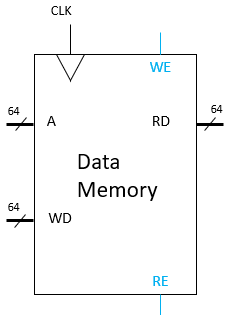
\includegraphics[width=0.3\linewidth]{Image/Data Memory.png}
    \caption{Data Memory}
    \label{fig:enter-label}
\end{figure}

\subsubsection{Implementation}
\textbf{Parameterization:}
\begin{itemize}
\item \textbf{Data Width:} The width of the data bus, which determines how much data can be read from or written to the memory in one operation. In the provided code, this is set to 64 bits.

\item \textbf{Address Width:} The width of the address bus, which determines the number of addressable memory locations. Here, it's set to 64 bits.
\end{itemize}
\textbf{Input/Output Interfaces:}
\begin{itemize}
\item \textbf{clk (input):} Clock signal to synchronize operations.
\item \textbf{memWriteEnable (input):} Control signal to enable writing to memory.
\item \textbf{memReadEnable (input):} Control signal to enable reading from memory.
\item \textbf{address (input):} 64-bit address bus specifying the memory location for read/write operations.
\item \textbf{writeData (input):} 64-bit data bus carrying the data to be written to memory.
\item \textbf{readData (output):} 64-bit data bus outputting the data read from memory.
\end{itemize}

\textbf{Memory Array:}

\begin{itemize}
\item The memory array is 128 bytes, organized as an array of 8-bit registers.
\end{itemize}

\textbf{Read and Write Operations:}

\begin{itemize}
\item Write operation should be synchronous with the clock signal.
\item Read operation should be combinational based on the control signal.
\item Data should be written and read in chunks of 64 bits, spread across 8 consecutive memory locations.
\end{itemize}

\textbf{Initialization:\textbf}
\begin{itemize}
\item The memory array should be initialized to zero during simulation.
\end{itemize}
\section{Decoder}

The decoder module is a crucial component in the control unit of a processor, responsible for interpreting 32-bit instructions and generating control signals that manage the processor's operations.
The inputs to the decoder module include a 32-bit instruction and a 64-bit program counter (pc). The instruction to be decoded comprises the opcode, function codes, and operand addresses, while the program counter indicates the address of the instruction. The outputs of the decoder include several control signals (\texttt{branch}, \texttt{memRead}, \texttt{memWrite}, \texttt{memToReg}, \texttt{aluSrc}, \texttt{writeReg}), ALU control signals (\texttt{aluOp}, \texttt{aluCtl}), register addresses (\texttt{readAddr01}, \texttt{readAddr02}, \texttt{writeAddr01}), the updated program counter (\texttt{newPC}, \texttt{curretPC}), and a 64-bit immediate value (\texttt{immidiateValue}).

\subsection{Truth Table}
The truth table below summarizes the control signals generated by the decoder module for each instruction type.
\setlength{\tabcolsep}{6pt} % Adjust as necessary
\begin{table}[h]
\centering
\setlength{\tabcolsep}{4pt} % Adjust as necessary
\begin{tabularx}{\textwidth}{|p{2.4cm}|p{2cm}|p{2cm}|X|X|X|X|X|X|}
\hline
\textbf{Instruction} & \textbf{ALUSrc} & \textbf{Mem to}\newline \textbf{Reg} & \textbf{Reg} \newline \textbf{Write} & \textbf{Mem} \newline \textbf{Read} & \textbf{Mem} \newline \textbf{Write} & \textbf{Branch} & \textbf{ALU} \newlinw \textbf{Op1} & \textbf{ALU} \newlinw \textbf{Op0} \\
\hline
R-format & 0 & 0 & 1 & 0 & 0 & 0 & 1 & 0 \\
\hline
ld & 1 & 1 & 1 & 1 & 0 & 0 & 0 & 0 \\
\hline
sd & 1 & X & 0 & 0 & 1 & 0 & 0 & 0 \\
\hline
beq & 0 & X & 0 & 0 & 0 & 1 & 0 & 1 \\
\hline
\end{tabularx}
\caption{Setting of the control lines is completely determined by the opcode fields of the
instruction.}
\end{table}

\subsection{Instruction Types}
The decoder module handles four instruction types: R-Type, Memory Load, Memory Store, and Branch instructions.

\textbf{R-Type Instructions}
R-Type instructions perform arithmetic and logical operations between registers. The control signals generated for R-Type instructions indicate no branching or memory access, with the ALU using register operands and writing back to the register file. Examples of R-Type instructions include ADD, SUB, AND, and OR. The ALU operations for R-Type instructions are specified by \texttt{aluOp} and \texttt{aluCtl} based on the function codes.

\textbf{Memory Load Instructions}
Memory Load instructions load data from memory into a register. The control signals for these instructions enable memory read, with the ALU performing address calculation and the data being written back to the register. An example of a Memory Load instruction is LW (load word). The immediate value for Memory Load instructions is extracted and sign-extended from the instruction.

\textbf{Memory Store Instructions}
Memory Store instructions store data from a register into memory. The control signals for these instructions enable memory write, with the ALU performing address calculation and no register write back. An example of a Memory Store instruction is SW (store word). The immediate value for Memory Store instructions is extracted from the instruction and combined into two parts.

\textbf{Branch Instructions}
Branch instructions perform conditional jumps based on register comparisons. The control signals for these instructions enable branching, with the ALU performing subtraction to compare register values. An example of a Branch instruction is BEQ (branch if equal). The immediate value for Branch instructions is extracted and sign-extended from the instruction.

\textbf{Control Signal Generation}
Control signals are generated based on the instruction's opcode. For R-Type instructions, the signals are set for arithmetic or logical operations with register operands. For Memory Load instructions, the signals enable memory read and data transfer to a register. For Memory Store instructions, the signals enable memory write from a register. For Branch instructions, the signals configure the ALU for comparison and enable branching. The ALU control signals (\texttt{aluOp} and \texttt{aluCtl}) are derived from the opcode and function codes. For R-Type instructions, ALU control is based on \texttt{funct7} and \texttt{funct3}. For Memory Load and Store instructions, the ALU is set to perform address calculation (addition). For Branch instructions, the ALU is set to perform subtraction for comparison.

\textbf{Immediate Value Extraction}
Immediate values are extracted and sign-extended to 64 bits for memory access and branch instructions, facilitating address calculation or branch target computation. This process ensures that the instructions are accurately interpreted and executed by the processor.


\subsection{Decoder Functioning}


\begin{itemize}
    \item The decoder module is responsible for interpreting the instruction and generating control signals for other components within a CPU. This functionality is depicted in the block diagram.
    \item \textbf{Instruction Fetch:} The 32-bit instruction, fetched from memory, serves as the input that needs to be decoded.
    \item \textbf{Program Counter (PC):} Holds the current address of the instruction being executed.
    \item \textbf{Opcode Decoder:} Extracts the opcode from the instruction to determine the type of instruction and generate the appropriate control signals.
     \item \textbf{Function Decoder:} Extracts the function codes (\texttt{funct7} and \texttt{funct3}) from the instruction to specify the particular operation (e.g., ADD, SUBTRACT, AND, OR) for R-type instructions.
    
\begin{figure}[H]
    \centering
    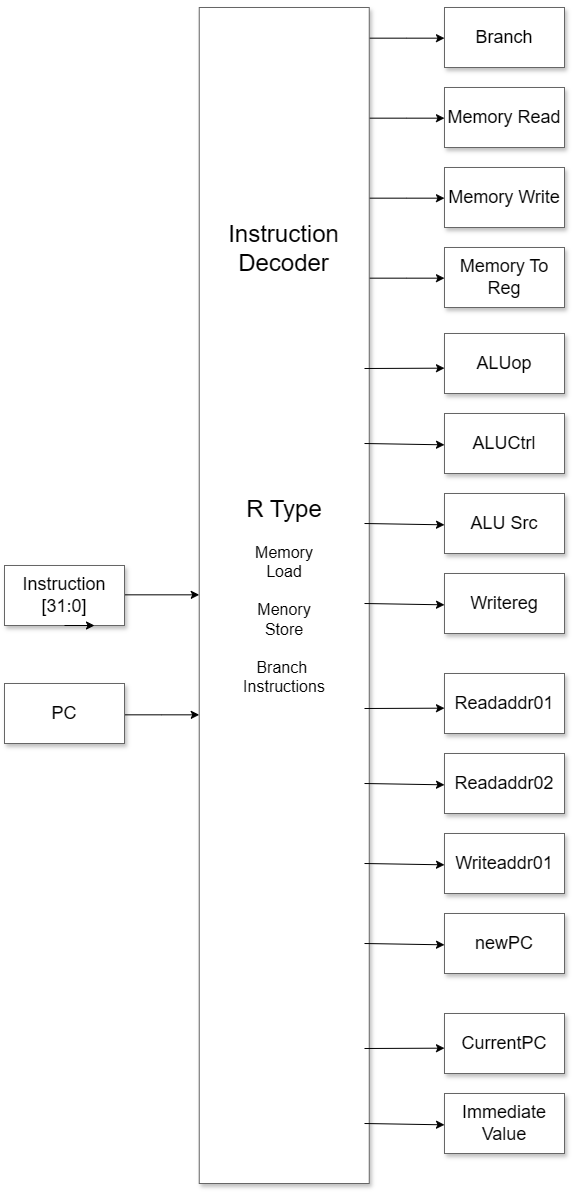
\includegraphics[width=0.95\textwidth, height=0.8\textheight]{Image/Decoder Block Diagram.drawio.png}
    \caption{Instruction Decoder}
    \label{fig: Instruction Decoder}
\end{figure}

   
    \item \textbf{Read Address 1 (rs1) and Read Address 2 (rs2):} Extract the respective fields from the instruction, specifying the source registers for the operation.
    \item \textbf{Write Address (rd):} Extracts the field indicating the destination register for the operation's result.
    \item \textbf{Immediate Value Extraction:} Handles the extraction of immediate values from the instruction for relevant operations.
    \item \textbf{Current PC:} Represents the address of the current instruction.
    \item \textbf{New PC:} Incremented by 4, points to the next instruction.
    \item \textbf{Control Unit:} Generates control signals based on the opcode, including signals for Branch, MemRead, MemWrite, MemToReg, ALUSrc, and WriteReg.
    \item \textbf{ALU Control Unit:} Produces ALU control signals (\texttt{ALUOp} and \texttt{ALUCtl}) derived from the opcode and function codes. Specific control signals such as Branch Control manage branching operations, Memory Read Control oversees memory read operations, Memory Write Control handles memory write operations, Memory to Register Control determines whether data from memory or the ALU is written to the register, ALU Source Control decides if the second ALU operand is a register value or an immediate value, and Write Register Control governs whether the result is written to a register.
    \item \textbf{Arithmetic Logic Unit (ALU):} Performs arithmetic or logical operations as specified by the control signals.
    \item \textbf{Register File:} Holds the CPU registers, interfacing with read and write addresses to access or store data.
    \item This comprehensive setup ensures the decoder module functions effectively, interpreting instructions and coordinating the necessary control signals for proper CPU operation.
\end{itemize}



\newpage
\section{Branch PC Generator}
The \texttt{branchPCGenerator} module is a crucial component in the control unit of a processor, implemented using Verilog, a hardware description language. This module determines the next value of the program counter (PC), which is essential for guiding the processor's instruction flow. It takes several inputs, including control signals and current state values, to decide whether to branch to a new address or continue sequentially. The primary inputs to this module are \texttt{branchControl}, \texttt{zeroFlag}, \texttt{newPC}, \texttt{curretPC}, and \texttt{immidiateValue}, while the output is the \texttt{nextPC}.

\begin{figure}[H]
    \centering
    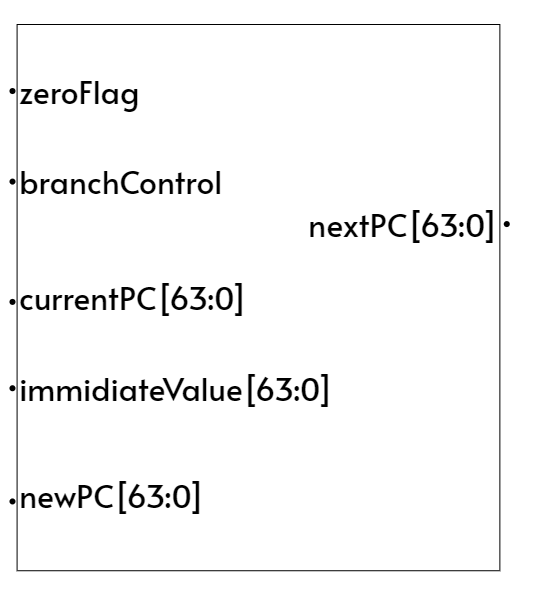
\includegraphics[width=0.3\textwidth, height=0.23\textheight]{Image/02_BPC.png}
    \caption{Branch PC generator}
    \label{fig:Branch PC generator}
\end{figure}

The inputs \texttt{branchControl} and \texttt{zeroFlag} are critical for branch decision-making. \texttt{branchControl} indicates whether a branch instruction is active, and \texttt{zeroFlag} reflects the outcome of a condition check, typically whether a computed result is zero. These signals are combined using a logical AND operation to produce the \texttt{branchDecision} signal. This signal is high only when both the branch control is asserted and the zero flag condition is met, indicating that a branch should be taken. 
\\ 
\hfill \break
The \texttt{nextPC} value is calculated based on the \texttt{branchDecision} signal. If \texttt{branchDecision} is high, indicating that a branch should be taken, \texttt{nextPC} is set to the current PC (\texttt{curretPC}) plus an immediate value (\texttt{immidiateValue}) shifted left by one bit. The left shift operation effectively multiplies the immediate value by two, a common technique used in instruction set architectures for byte addressing with word-aligned instructions. This operation ensures that the processor can jump to the correct instruction address specified by the branch. 
\\ 
\hfill \break
If \texttt{branchDecision} is low, indicating that the branch condition is not met, the \texttt{nextPC} is set to \texttt{newPC}, which represents the next sequential instruction address. This conditional assignment, resembling a multiplexer function, ensures that the processor continues to execute instructions in the correct order, either by branching to a new address or moving to the next sequential address. Thus, the \texttt{branchPCGenerator} module enables efficient control flow management within the processor, ensuring that branch instructions are correctly handled based on the given conditions.



\newpage
\section{Top Level}

\subsection{Introduction}

In this section, we integrate all previously explained design elements to create a unified single-cycle processor. The top-level module includes specific multiplexers labeled as M1, M2, and M3. M1 controls the datapath for the second operand of the ALU, M2 manages the write-back operation to the register file, and M3 adjusts the datapath of the PC register during flash operations. These multiplexers are crucial as they enable the processor to adapt its datapaths based on the instruction being executed, allowing a variety of operations to be performed. We will also understand the instruction memory flash mechanism in detail.
\\ 
\hfill \break
This section focuses on implementing the single-cycle processor's datapath flow described in the product overview. It will detail how different instruction classes are executed, emphasizing the role of these multiplexers in enabling diverse operations within the processor.
\begin{itemize}
  \item Datapath for R-Type instructions.
  \item Datapath for load/store instructions.
  \item Datapath for branch-if-equal instruction.
\end{itemize}

\subsection{Datapath for R-Type instructions}

The figure below shows the datapath operation (Highlighted in red) for an R-type instruction such as \texttt{add x1, x2, x3}. Although everything occurs in one clock cycle, we can think of several steps to execute the instruction.

\begin{figure}[H]
    \centering
    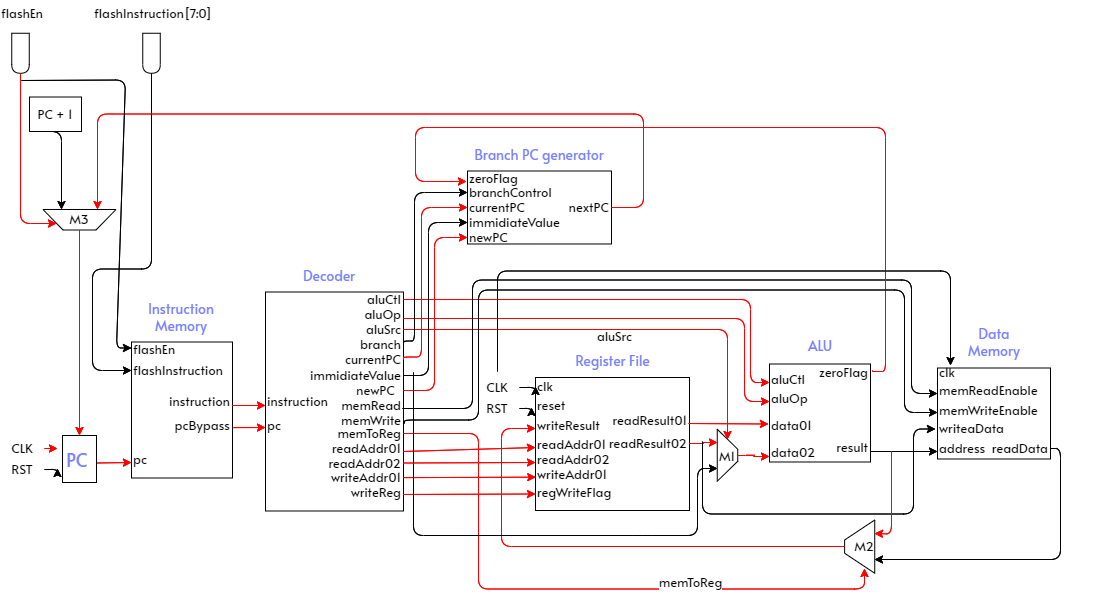
\includegraphics[width=0.95\textwidth, height=0.4\textheight]{Image/01_Rtype.png}
    \caption{R-Type Datapath}
    \label{fig:R-Type Datapath}
\end{figure}


\begin{itemize}
  \item On each rising edge of the clock pulse, if the processor is not in flash mode (flashEn is zero), the PC increments by 4.
  \item The instruction located at the updated PC (oldPC + 4) is fetched from the instruction memory and sent to the decoder for decoding. This process generates necessary signals and addresses required for executing the instruction.
  \item  For the current instruction "add x1, x2, x3", values from register file addresses x2 and x3 are fetched and sent to the ALU.

  \item  As "add" is an R-Type instruction, aluSrc signal is zero, and M1 mux directs readResult02 to the ALU as the second operand.
  \item The ALU performs an arithmetic addition based on signals aluCtl and aluOp from the decoder. The resulting value is written back to register file location x1. memToReg flag is zero, and regWriteFlag is High, enabling this write operation.

  \item Since the branch signal is zero, the branch PC generator forwards the newPC (oldPC + 4) to nextPC. This updated value is loaded into the PC register at the next rising edge of the clock cycle.
\end{itemize}


\subsection{Datapath for load/store instructions}

The figure below shows the datapath operation (Highlighted in red) for a load instruction such as \texttt{ld x1, offset(x2)}. Although everything occurs in one clock cycle, we can think of several steps to execute the instruction.

\begin{figure}[H]
    \centering
    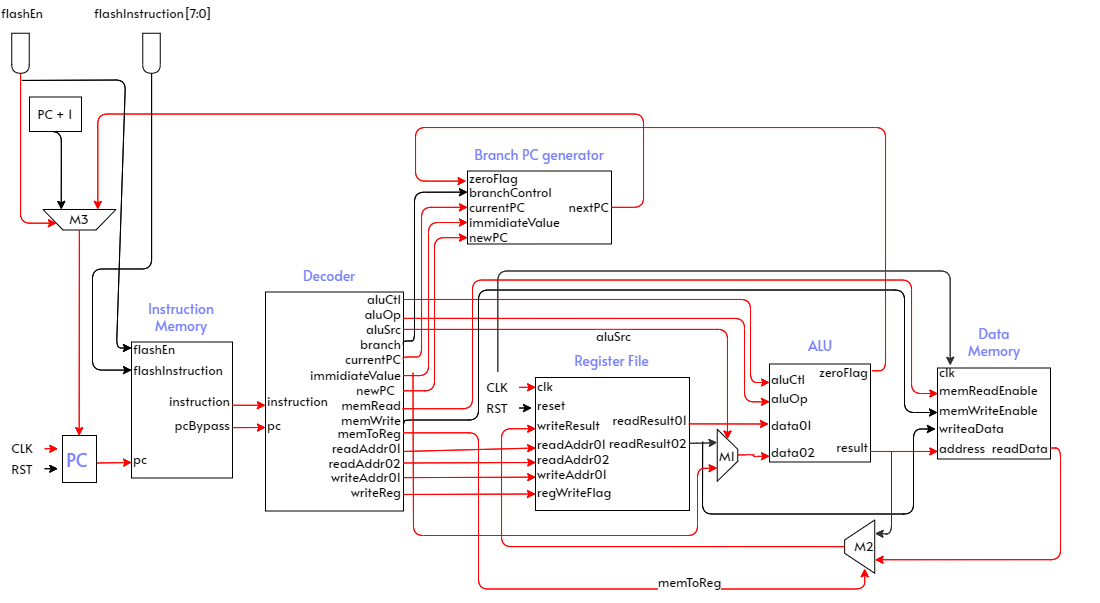
\includegraphics[width=0.95\textwidth, height=0.4\textheight]{Image/02_load.png}
    \caption{load/ store Datapath}
    \label{fig:load/ store Datapath}
\end{figure}

\begin{itemize}
  \item At each rising edge of the clock pulse, the PC increments by 4 when the processor is not in flash mode (flashEn is zero).
  \item The instruction located at the new PC (oldPC + 4) is fetched from the instruction memory and passed to the decoder for decoding. This process generates the necessary signals and addresses required for executing the instruction.

  \item For the current instruction "ld x1, offset(x2)", the value from register file address x2 is sent to the ALU. The ALU's second operand is a 12-bit immediateValue from the decoder, as aluSrc signal is High, and mux M1 adjusts the datapath accordingly compared to the previous instruction.

  \item The ALU adds these operands as directed by signals aluCtl and aluOp, producing the memory address from which data needs to be fetched.

  \item Since the memory read operation is clock-independent, the fetched data is written back to the register file during the falling edge of the same clock cycle. Here, mux M2 alters the datapath for the write-back operation to the register file, since memToReg signal is High. The fetched value is stored in register x1 of the register file.

  \item Meanwhile, with branch signal at zero, the branch PC generator forwards newPC to nextPC (oldPC + 4). This updated value is loaded into the PC register at the next clock cycle's rising edge.
\end{itemize}

Store operations will also have an almost similar datapath to store data from the reg file into the data memory.

\subsection{Datapath for branch-if-equal instructions}

The figure below shows the datapath operation (Highlighted in red) for a branch-if-equal instruction such as \texttt{beq x1, x2, offset}. It operates much like an R-format instruction but the ALU output is used to determine whether the PC is written with PC + 4 or the branch target address. Although everything occurs in one clock cycle, we can think of several steps to execute the instruction.


\begin{itemize}
  \item  During each rising edge of the clock pulse, the PC increments by 4 when the processor is not in flash mode (flashEn is zero).
  \item The instruction located at the updated PC (oldPC + 4) is fetched from the instruction memory and forwarded to the decoder for decoding. This step generates the necessary signals and addresses required to execute the instruction.

  \item Two registers, x1 and x2, are accessed and read from the register file.
  \item The ALU subtracts one data value from another, both obtained from the register file. If the result of this operation is zero, the zeroFlag is set High. If the branch flag is also High, indicating a branch instruction, the branch PC generator computes the branch target address by adding the current PC value to the sign-extended immediateValue (offset) extracted from the instruction (12 bits, left shifted by one).
  \item The new branch target address is written into the PC register during the rising edge of the next clock cycle. The instruction memory then retrieves and executes the instruction located at this branch target address. This process occurs independently of the clock due to the nature of instruction memory read operations.
\end{itemize}

\begin{figure}[H]
    \centering
    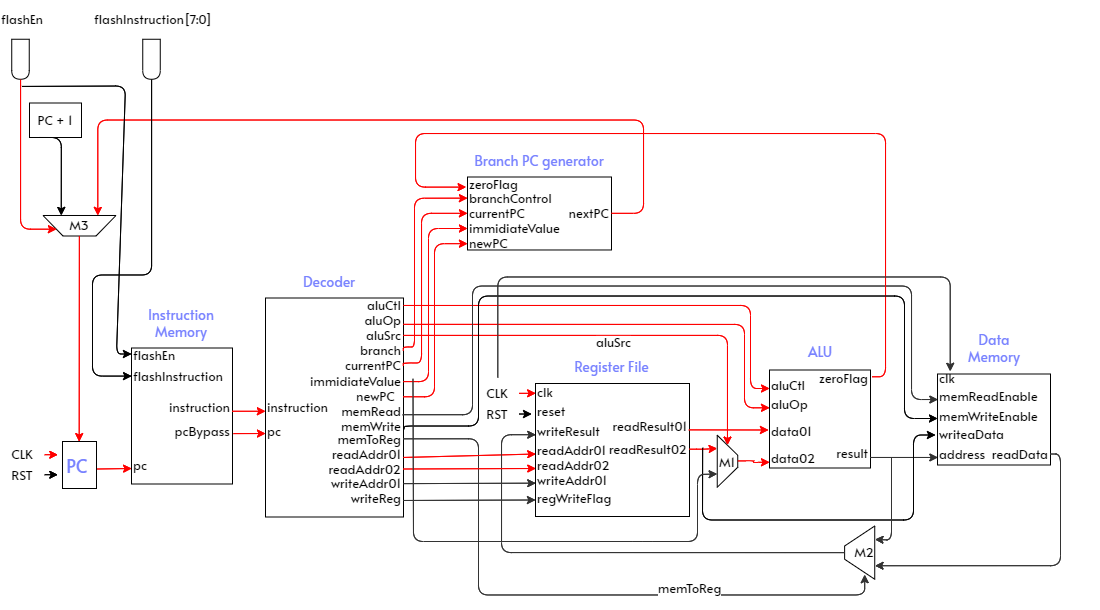
\includegraphics[width=0.95\textwidth, height=0.4\textheight]{Image/03_beq.png}
    \caption{Branch-if-equal Datapath}
    \label{fig:Branch-if-equal Datapath}
\end{figure}

These operations encompass all potential datapaths the processor can generate, providing a comprehensive understanding of the functional principles underlying the single-cycle RISC-V processor.


\subsection{Datapath for processor flash operation}

The diagram below illustrates the datapath operation (highlighted in red) for the processor's instruction memory during a flash operation. In the RISC-V architecture, each instruction is 32 bits wide, while the instruction memory operates on a byte-addressable basis. Initially, a hex file must be generated from high-level languages or assembly code using a dedicated toolchain. Once this hex file is prepared, the processor can be flashed by simulating the process typically handled by an onboard debugger like JTAG or a TAP Controller.
\\ 
\hfill \break
In this scenario, although no specific debugger is employed, the process involves writing one byte at the corresponding PC location in the instruction memory from the hex file. If the flashEn signal is High, the PC increments by one at the rising edge of each clock cycle, enabling the loading of one byte of instruction per clock cycle.

\begin{figure}[H]
    \centering
    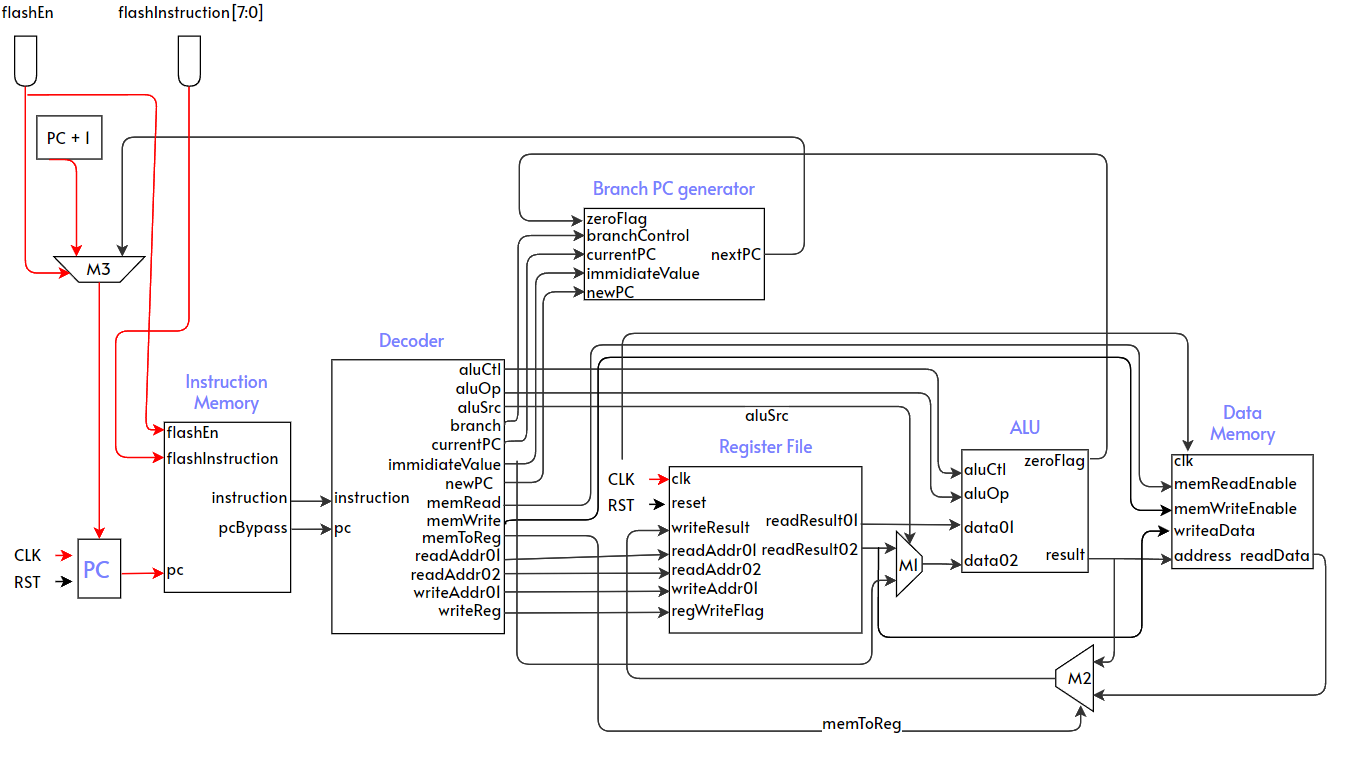
\includegraphics[width=0.95\textwidth, height=0.4\textheight]{Image/04_flash.png}
    \caption{Flash Datapath}
    \label{fig:Flash Datapath}
\end{figure}

After completing the flashing operation, deactivate the flashEn signal and reset the processor. Subsequently, the processor will transition to normal mode and begin executing the instructions stored in the instruction memory that were loaded during the flashing process.



\newpage
\customchapter{Simulation results}
\section{Flash instruction memory}

The diagram below demonstrates the procedure of flashing the instruction memory. Throughout this process, the Program Counter (PC) advances by one on each clock cycle, and a byte of data from the hex file, containing instructions, is stored in the byte-addressable instruction memory. Flashing is active only when the flashEn signal is high and the reset signal is low, as indicated in the output. This operation of flashing takes about 290 nanoseconds to write 28 bytes of 7 RISC-V instructions into the instruction memory.

\begin{figure}[h!]
    \centering
    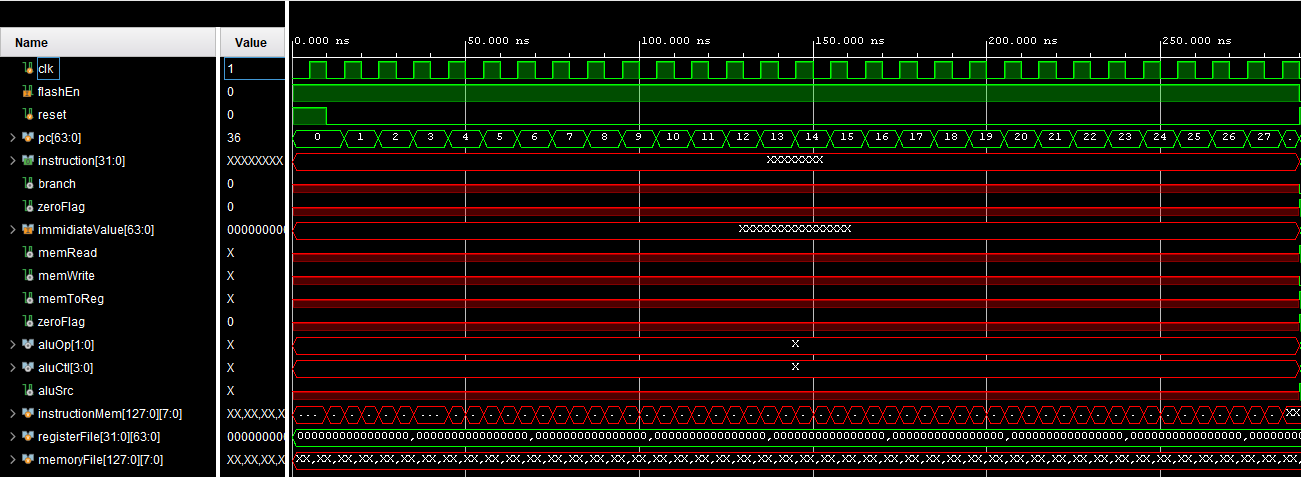
\includegraphics[width=0.9\textwidth, height=0.3\textheight]{Image/01_Sim.png}
    \caption{Instruction Memory Flashing Process}
    \label{fig:flash_memory}
\end{figure}

\section{Processor simulation}

After the instructions have been flashed into memory, the processor can be reset, causing the PC to reset to zero. Subsequently, the processor begins fetching instructions from the memory starting at address zero. This behavior is depicted in the image below. To facilitate explanation, the following timelines are considered:

\begin{figure}[h!]
    \centering
    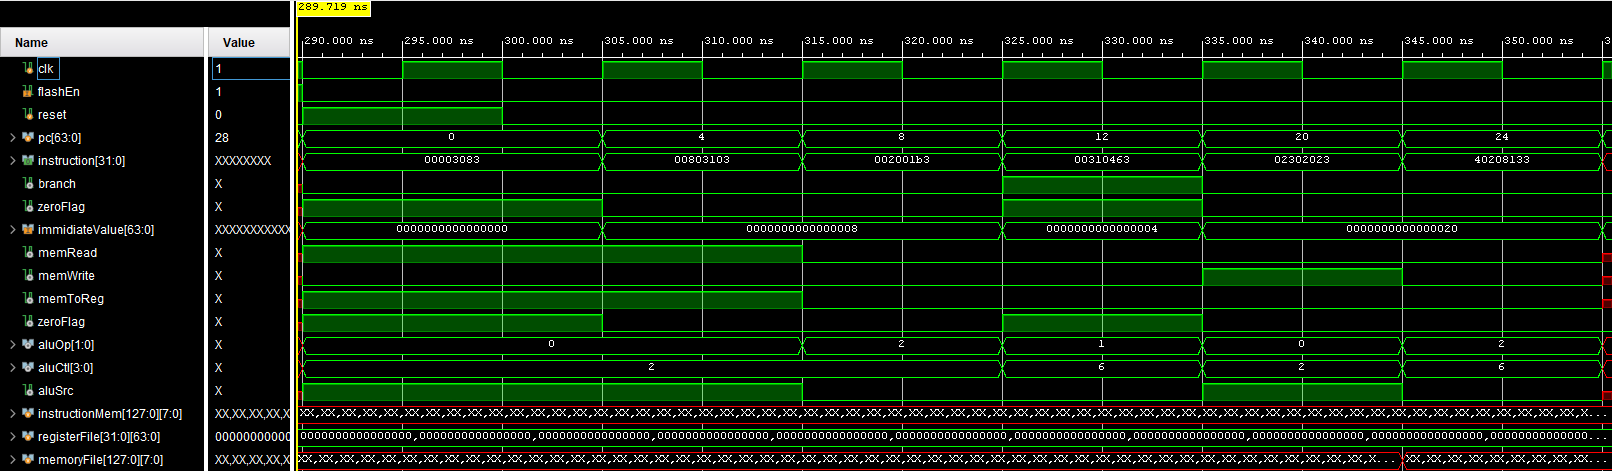
\includegraphics[width=1.0\textwidth, height=0.23\textheight]{Image/02_sim.png}
    \caption{Processor Simulation}
    \label{fig:processor_simulation}
\end{figure}

\begin{itemize}
    \item \textbf{Time Stamp (290ns – 300ns):} The reset signal gets pulsed, the PC becomes zero, and fetches the first instruction \texttt{ld r1 0(r0)} where \texttt{r0=0} with the hex code of \texttt{0x00003083} gets executed which fetches a double word from \texttt{0x00} data memory location into the \texttt{r1} register of the register file.
    \item \textbf{Time Stamp (300ns – 310ns):} Now \texttt{PC=4} and the next instruction gets fetched \texttt{ld r2 8(r0)} where \texttt{r0=0} with the hex code of \texttt{0x00803103} gets executed which fetches a double word from \texttt{0x08} data memory location into the \texttt{r2} register of the register file.
    \item \textbf{Time Stamp (310ns – 320ns):} Now \texttt{PC=8} and the next instruction gets fetched \texttt{add r3 r2 r0} with the hex code of \texttt{0x002001b3} gets executed which adds the data present in \texttt{r0} and \texttt{r2} registers and then stores the result in the \texttt{r3} register.
    \item \textbf{Time Stamp (320ns – 330ns):} Now \texttt{PC=12} and the next instruction gets fetched \texttt{beq r3 r2 4(offset)} with the hex code of \texttt{0x00310463} gets executed which checks if \texttt{r3==r2}, if yes then it gets branched to target address \texttt{(currentPC+4) + 4(offset)}. So \texttt{newPC = 20}. Also, observe imidiateValue during branch.
    \item \textbf{Time Stamp (330ns – 340ns):} Now \texttt{PC=20} and the next instruction gets fetched \texttt{sd r3 32(r0)} with the hex code of \texttt{0x02302023} gets executed which stores data present in \texttt{r3} at \texttt{r0+32}.
    \item \textbf{Time Stamp (340ns – 350ns):} Now \texttt{PC=24} and the next instruction gets fetched \texttt{sub r2 r2 r1} with the hex code of \texttt{0x40208133} gets executed which subtracts \texttt{r2 – r1} and stores back data into \texttt{r2}.
\end{itemize}







\newpage
 \begin{thebibliography}{9}
	
	\bibitem{ref1} 
	 Computer Organization and Design: The Hardware/Software Interface, February 27, 2017,RISC-V Edition,by Hennessy, J. L.  
  
	\bibitem{ref2} 
	Digital Design and computer architechture by David Money Harris, May 2, October 2008. 
	
	
\end{thebibliography}


\end{document}